\textbf{\LARGE{Part one: Design Project}}
\todo[inline]{Part one is a design project report as described
    in the coursebook. The audience for this is the companies
    management. See e.g.\ page 186ff.
    Length between 25-30pp}

\section{Objective}

\subsection{Objective of the design project}
\todo[inline]{Recap of the requirements from the manager, and what goals 
    the system is designed to fulfill}
The focus of the design project is to improve upon the booking process used by 
\gomonkey. The booking process is currently very manual and only ever handled by 
the manager. The manager said that: 

\begin{quotation}
I don't dare letting my employees handle the bookings!

\em - Michel Pascual, manager and owner of \gomonkey, 15.10.2013
\end{quotation}

He is afraid they will make mistakes, since the process is complex and not very 
well documented. Some bookings may also contain cases which the manager is not 
yet sure of how should be handled, and thus needs an authority to handle and  
produce a best practice for \gomonkey{}. While the manager does spend a lot of
time handling bookings, this takes time from actually evolving the business.
The goal of the design project is to put the booking process into a 
well defined system and reduce the complexity and time required for handling
incoming bookings. This will reduce the workload put on the manager, thus 
empowering him to focus on other areas of the business.

\subsection{Results from the in-line analysis}
The in-line analysis is meant to help us understand the environment in which 
the company is situated, the business strategy of the company, and what work
domains are defined within the business. This will help the designers to
better understand the reasoning behind current work practices and how to 
solve the problems that arise. The most noteable parts of the results from 
the in-line analysis are the business strategy and the overview of the work 
domains of \gomonkey{}.

\subsubsection{Business strategy}
The business strategy of \gomonkey{} was not written down before we started the
project, so we had to construct and interpret on our perception of the company.
This changed during the course of the design project, and this is the final 
result:

\begin{enumerate}
	\item Become a self-sustainable climbing company with customers on a daily basis.
	\item Minimize time requirements pr.\ booking/customer.
	\item Minimize staff requirements to keep costs low.
	\item Increase sales (Such as selling food, drinks, etc.).
	\item Provide better and more comprehensive services than competitors.
\end{enumerate}

While these are not easily quantifiable, and thus are not a very suitable list
for a business strategy, it will work for this purpose. Whenever we do suggest
a change for the company, we should be able to, directly or indirectly, point to
a specific point in the business strategy.

\subsubsection{Work domains}
The company, while selling climbing sessions as a service, clearly does other
things that does not directly add value, but a necessary nonetheless.		%this is spelled correctly! nonetheless
While interviewing and observing the company, we mapped out those areas of 
work, and the result can be seen in \autoref{table:workdomain}.

\begin{table}[H]
    \centering
\begin{tabular}{ |l|l| }
        \hline
        Work domain & Example work processes \\ \hline
        \multirow{4}{*}{Booking Flow} 
            & Registering received bookings \\
            & Checking payment status \\
            & Informing customers prior to arrival \\
            & Receiving customers \\
        \hline
        \multirow{3}{*}{Employee Schedule} 
            & Scheduling shifts \\
            & Swapping shifts \\
            & Time registration \\
        \hline
        \multirow{2}{*}{Economy and bookkeeping} 
            & Payment during booking \\
            & Invoice after visit \\
        \hline
        \multirow{2}{*}{Inventory Management} 
            & Maintenance of inventory \\
            & Stock control of equipment \\
        \hline
        \multirow{2}{*}{Marketing} 
            & Advertising \\
            & Offers and discounts \\
        \hline
\end{tabular}
\caption{List of work domains and example work processes in the specific work domain}
\label{table:workdomain}
\end{table}

This makes us more aware of what the company does. This can be used to further 
explore what processes exists and map exactly how they are performed. But more 
important, this allows us to ignore certain parts of the company that are not 
related to the problems we are trying to solve with a system. An effort focused
on a single work domain is bound to get into more details, and thus yield a 
better result.


\subsection{Results from the in-depth analysis}
\todo[inline]{Observations, standard systems, work practices}

The in-depth analysis is meant to help us understand exactly how and why the 
existing processes work as they do. This was done by observing the processes,
analysing documents and correspondance, and mapping out exactly what work 
practices resulted in problematic situations. In the following section we describe the 
work practies we found, and what problems were discovered. When we knew the
business practices and related problemss, we surveyed the market for a useable 
standard system, which is described later in this section.

\subsubsection{Work practices and their problems}

\begin{description}
\item[Initial Booking]
A potential customer which has landed on the website can initiate a booking
by accessing the booking form. He then has to fill in his name, e-mail, phone number, 
the desired booking date and time, the number of persons that will be joining and their
age span along with any additional notes he might have. The interface isn't state of the art 
and does not provide error recoverability, which is a great usability concern and is 
strongly encouraged. After the user has managed to fill in the form, he is taken to a confirmation
page and two emails are sent: one to the manager with the booking information from the form and
one to the customer informing them that \gomonkey  has received their booking request. The process
cand be followed in \autoref{fig:customer}.

\begin{figure}[htbp]
    \centering
        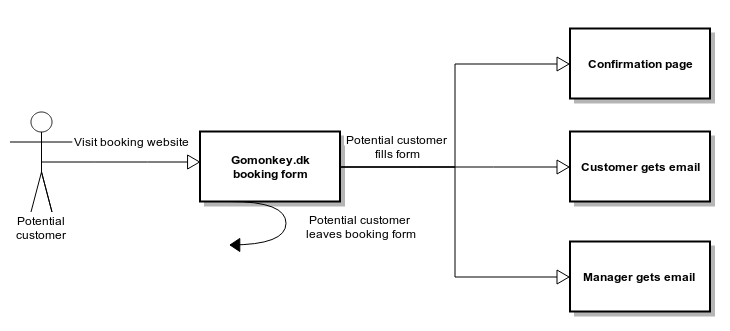
\includegraphics[width=\textwidth]{figures/customer.png}
            \caption{Overview of an initial booking.}
        \label{fig:customer}
\end{figure}

\item[Processing a booking]
The manager reads the booking request email and contacts the customer to provide additional
information if the booking request does not have all the required data. The manager and the 
customer communicate over email until both parties are satisfied with the terms of the booking.
An overview of this can be seen in \autoref{fig:manager}. This manual gathering of additional
booking information can be avoided by building a more complex booking system. After the customer
has supplied all the requested information, the manager then enters the information in Google
Calendar, linking the email with the event. A confirmation email is sent to the customer to
inform him the booking is scheduled.

\begin{figure}[htbp]
    \centering
        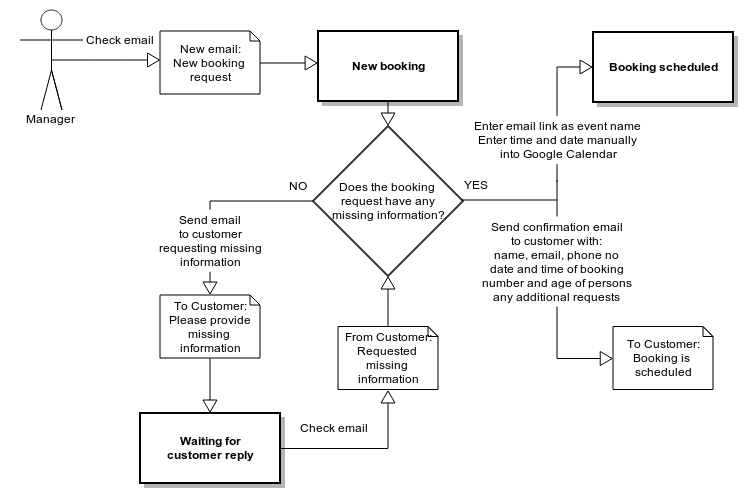
\includegraphics[width=\textwidth]{figures/manager.png}
            \caption{Overview of a booking processing.}
        \label{fig:manager}
\end{figure}

\item[Processing payment]
As seen in \autoref{fig:payment}, the manager is also the one who is processing payments. Every two days,
he logs into his netbank account and associates transactions with their respective bookings in Google Calendar. 
Sometimes customers forget to write their name on their transaction and that causes some distress as the
manager cannot identify the customer. Having to do everything manually leaves room for human error,
a situation which should be avoided. Finally, the manager colors the event associated with the booking
in Google Calendar and changes its description to reflect payment status.

\begin{figure}[htbp]
    \centering
        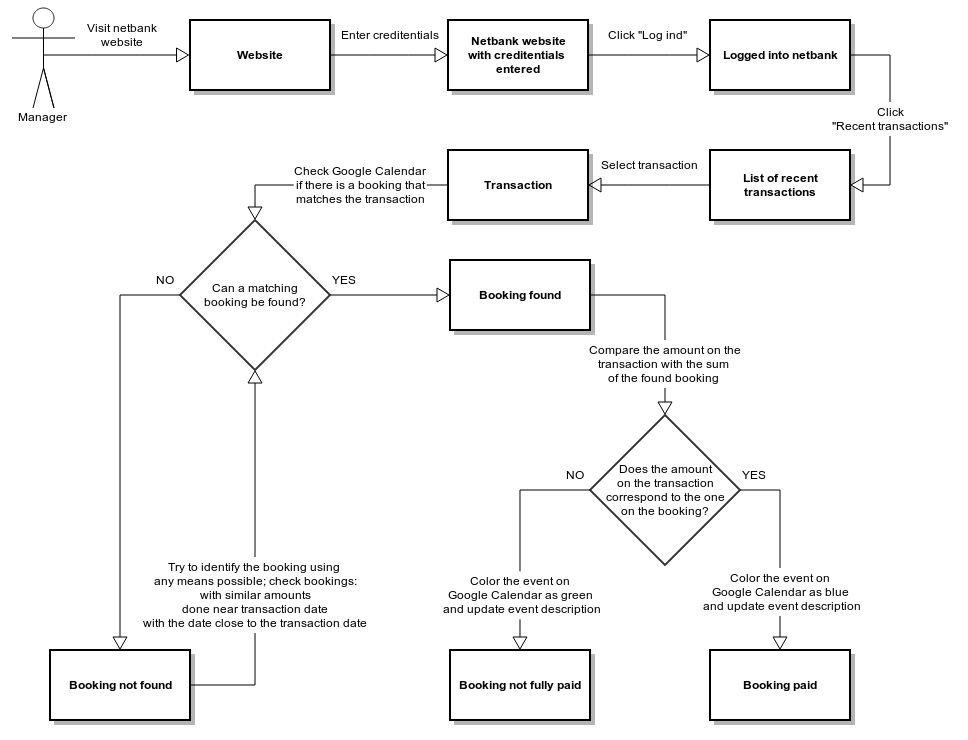
\includegraphics[width=\textwidth]{figures/payment.png}
            \caption{Overview of payment processing.}
        \label{fig:payment}
\end{figure}

\item[Handling booked customers]

\begin{figure}[htbp]
    \centering
        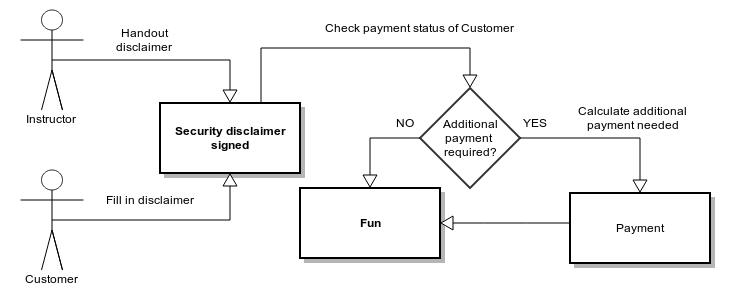
\includegraphics[width=\textwidth]{figures/handling.png}
            \caption{Overview of customer handling}
        \label{fig:handling}
\end{figure}
ref \autoref{fig:handling}

\end{description}

\subsubsection{Finding a suitable standard system}
It is often a good solution to find a standard system which solves the problem 
at hand. This can save a lot of time and money, and can quickly solve a complex
problem.
We compiled a list of possible standard systems and isolated three very possible
candidates. After deep testing sessions of all systems, we realized that none
of them fulfill the defined requirements in the design project. The testing
session included creating a free temporary booking system. All systems tend to 
have this feature, so potential customers can evaluate the usefullness prior to 
paying. Attempts were then made to setup the system to support the needs of
\gomonkey{}, and after testing the usefullness of the result, we could conclude
upon the advantages and disadvantages of implementing the system.

\begin{description}
\item[SuperSaaS]
We decided not to use SuperSaaS, since the booking doesn’t support the required 
fields for the booking. A `form' can be attached to a booking after submitting 
initial information (intial information being the date and time of booking, 
name, phone number and email address), and this 
form can include extra information about amount of people in each age group, the
type of customer and food. This information can only be seen with two clicks 
from the calendar overview, thus making it impossible to get a good overview of 
how `available' a time slot is.

Furthermore, it is not possible to calculate a price based on the custom fields 
in the form, and as such, the system cannot ask for a deposit so we will still 
need another payment processor.

\item[onlinebooq.dk]
The second promising booking system was onlinebooq.dk. They support selling 
`services', but unfortunately they only support selling one of each servive.
This can be seen in \autoref{fig:onlinebooq} as the checkbox, next to the 
service in question. This makes it useless for \gomonkey{}, since the price is 
calculated from the amount of people utilizing each service. It does support 
paypal and quickpay, but this doesn't matter if we cannot calculate the price 
correctly.

\begin{figure}[htbp]
    \centering
        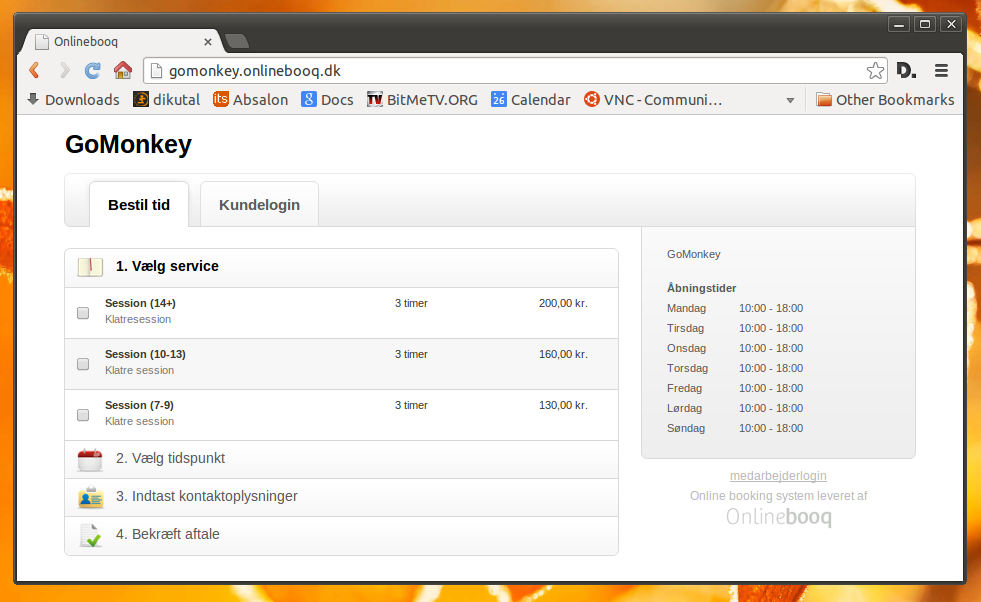
\includegraphics[width=.8\textwidth]{figures/onlinebooq.png}
	    \caption{Screenshot from testing onlinebooq.dk.}
        \label{fig:onlinebooq}
\end{figure}
		

\item[Cyberbooking]
The last booking system we tested was Cyberbooking. They have two types of 
calendars, one which supports one resource (e.g.\ a hairdresser) who can only
perform one service at a time. The other type supports booking slots on 
predefined events, (e.g.\ a fitness session) and the events are set by the 
company. None of these types can help \gomonkey{} with the booking process,
since the amount of resources aren't limited to one group of customers, and 
the times of bookings are very flexible.
\end{description}

While none of the systems fit with \gomonkey{}'s business, we attempted
to find a way to adjust \gomonkey{}'s business to the systems. This was not 
successful and would alter the work practices in a very negative way.


\section{The coherent vision}
The coherent vision we suggest here is based on the results from the in-line 
analysis and in-depth analysis. The vision is a suggestion for a system design, 
along with descriptions of any expected organizational additions and changes 
resulting from implemeting the system. It also includes reflections upon 
required qualifications of anyone who will have to interact with the system
and what advantages and disadvantages this will enforce thoughout the company.
Finally, it includes some financial figures and an implementation plan. This 
should give the required knowledge of the system to perform an informed choice
on wether to start the project.

\subsection{Technology and systems}
This section will describe the system itself, what it does and how it looks,
along with what is required to keep the system running. This is intended to 
help building the system, should the project be initiated.

\subsubsection{IT systems and platform}
The owner of \gomonkey{} insists that the main website continues to run on the 
WordPress which is hosted with One.com. This is a fine solution, and will make
sure that the website maintains it's current, existing Google page-rank.

Further, it is necessary to have a server for hosting the new system, with 
access to a database and a webserver. This is not achievable on the server from 
One.com, so another will have to be found. It will be sufficient to have 
interfaces to a database and a webserver, but it is optimal to have root acess
to the server.

The server can run any operating system which supports a database and a 
webserver, but preferably a free one, to avoid the costs of the license for a 
proprietary system.

Additionally, there will still be parts of the original system which remain. 
The scheduling and journaling of staff will still be hosted in the company's 
Google Drive. 

\subsubsection{Components, functions and interface}
\todo[inline]{Pictures of mockup and descriptions of how it works}

\subsection{Work organization}
\todo[inline]{Do we change how the work organization is organized, are there
someone someone with new responsibilities? Can someone potentially do some 
of the managers work?}

\subsection{Qualification needs}
\todo[inline]{Does the system require any education? The manager will probably
need to tell about the new system to the instructors, and the manager will have
to be `taught' how to use the new system.}
	
\subsection{Advantages and disadvantages}
\subsubsection{Business- and IT strategies}
\todo[inline]{How the system will help reach the goals described in the
    business- and IT strategies.}
\begin{description}
\item[Advantages]

\item[Disadvantages]
\end{description}

\subsubsection{Groups of staff and their relations}
This section describes how the coherent vision will help the staff do their 
job, and what drawbacks there may be. 

\begin{description}
\item[Advantages]
The proposed system will help the employees in several ways. It will be an
advantage for the instructor at work to have a more of the needed information
at hand. This will make for a less error prone handling of customers. The 
decifit price will be available to the instructor, instead of having to 
calculate the price manually. Further, the situation where a customer paid on 
the day and thus the instructor can't see the paid amount will completely be 
avoided, since we utilize payment processors with instant transaction 
confirmations.

The manager will have more time to spend on the employed staff, and this will
help building stronger relations with the employees. This will be a
good way to increase the joy with which the whole company works, and increase
the chance for having employees with much experience because they like their 
job, their colleagues and their manager.

\item[Disadvantages]
The manager is very invested in the system, and will want the employees to 
use the system quickly. The instructors may be less ready for the change and may
oppose spending time learning a new system. This can be avoided by making sure 
the instructors understand why the system is necessary and how it can help them 
do their work.
\end{description}

\subsubsection{Customers}
This section describes how the results of implementing the coherent vision will 
effect the user experience of customers in both positive and negative 
directions.

\begin{description}
\item[Advantages]
From the customers perspective, the improved interface will add to a pleasant
user experience. Previously, a lot of communication was very cumbersome, but 
with the new system, much of the communication is no longer needed, since the
topics discussed are supported by the new system. 

The reduced amount of cumbersome communication and easily understandable system
will also be partly visible  for the customer, since the company will seem more
professional, and the staff will be happier to welcome the customers upon 
arrival at \gomonkey.

The pleasant user experience will make sure the customer focuses on the kernel
business, the treetop climbing course, instead of the necessities of a booking.
This will lead to customers being more inclined to suggest visiting the park
to friends and family. 

\item[Disadvantages]
The reduced amount of cumbersome communication may lead the the booking process having
a less personal feeling for the customer. Knowing that you are writing with
another human being that actually caters for your specific needs is a very 
powerful tool, but it is also very time consuming for the company. This may
result in a more systematic and less personal interaction with \gomonkey, which
may or may not reduce the customers firsthand experience.
\end{description}


\section{Finances and costs}
The financial part of the system is not a big part of the analysis but it is
definitely an important part of being able to perform the, previously mentioned,
informed choice about wether to begin the design project or not.

We here suggest an estimate of how much we believe the system will cost. This
is based on the design teams knowledge of pricing similar systems and their 
prior experiences with such projects. 

To build the system it is necessary to hire a programmer and a graphics artist.
It is also necessary to have a server running permanently, hosting the system. 
The prices of those are as follows:

\begin{itemize}
\item Front-end programmer, \textbf{500DKK/hour}
\item Graphics artist, \textbf{500DKK/hour}
\item Server hosting, \textbf{100DKK/month}
\end{itemize}

We estimate the following time requirements:

\begin{itemize}
	\item 30 hours of a programmer, to turn mockups into an initial prototype and integrate with the existing site.
	\item 10 hours of a graphics artist in total, to create art assets for the website.
\end{itemize}

This brings the total cost of such a venture to \textbf{20.000DKK} plus, for the 
development of the system. During the development phase, the server hosting
fees will also have to be paid, and is added over the course of development.

After the development period, the server hosting fee will still have to be paid
for as long as the system must remain online and useable. 

Maintenance will also be necessary once in awhile, mostly to get security 
updates for used technologies. This will amount to approximately 10 hours year, 
and will amount to \textbf{5.000DKK/year}.


\section{Implementation strategy and plan}
\subsection{Technical implementation}
\subsection{Organizational implementation}

\section{Recommendations and priorities}

\newpage
